\chapter{Planificación}
.
\section{Metodología utilizada}
Para el desarrollo de esta app, usaré una metodología ágil tipo SCRUM. He decidido usar esta porque me permite corregir fallos en la velocidad diseño y/o planificación de forma eficiente y sin dañar el producto final.\\

Las reuniones con la tutora serán las sprints review.
\section{Temporización}

La temporización la hice el dían 25 de marzo del 2025, la entrega del producto(este TFG) sería el 16 de junio de 2025,
es decir, 83 días, o lo que es lo mismo, casi 12 semanas. Si un sprint son 2 semanas, tengo entonces 6 sprints hasta la entrega final.\\
La iteración 0 la voy a usar para diseño de pantallas y repasar las funcionalidades de la app .La idea a priori sería separar la app en varios módulos y centrar cada sprint en un módulo:
\begin{itemize}
	\item Diagramas de la app y ejercicios
	\item Rutinas, usuarios y sesión
	\item Datos que ingresa el usuario
	\item Flujo entrenamiento
	\item IA
	\item Smartwatch
\end{itemize}

\section{Seguimiento del desarrollo}
\subsection{Iteracion 0}
En esta primera iteración me centré en terminar todos los diseños de la app, sobretodo busqué que fueran lo más accesibles posible. Támbién concreté mi product backlog, quedándome con 24 historias de usuario, algunas de estas tienen tareas segundarias dentro de ellas:
\begin{itemize}
    \item SCRUM-1: Registrar peso por día
    \item SCRUM-2: Establecer peso objetivo
    \item SCRUM-3: Insertar/Borrar/Modificar ejercicio de la lista
    \item SCRUM-4: Buscar rutina en la lista del usuario
    \item SCRUM-5: Sustituir un ejercicio por otro en la rutina
    \item SCRUM-6: Insertar/Borrar/Modificar rutina
    \item SCRUM-7: Poner una meta en cada ejercicio
    \item SCRUM-8: Graficar los datos de los ejercicios
    \item SCRUM-9: Revisar datos para ver si el descanso es necesario
    \item SCRUM-10: Enseñar datos de una rutina a descargar
    \item SCRUM-11: Compartir mi rutina
    \item SCRUM-12: Guardar las repeticiones y series de todos los ejercicios de un entrenamiento
    \item SCRUM-13: Dar una valoración al entrenamiento en base a la marca actual y meta del usuario
    \item SCRUM-14: Monitorizar pulso en tiempo real
    \item SCRUM-15: Medir pulso en reposo para hacer comparaciones con los datos de los ejercicios
    \item SCRUM-16: Avisar de alguna anomalía en el pulso de forma suave
    \item SCRUM-17: Obtener calorías quemadas
    \item SCRUM-18: Comprobar el equilibrio nervioso del usuario
    \item SCRUM-19: Realizar el flujo del entrenamiento
    \item SCRUM-20: Conectar con la IA para empezar diálogo
    \item SCRUM-21: Crear/Borrar mi usuario
    \item SCRUM-22: Resumir datos
    \item SCRUM-23: Iniciar/Cerrar sesión
    \item SCRUM-24: Medir SpO2
    \item SCRUM-25: Interpretar constantes
\end{itemize}
\subsubsection{Sprint review}
En este sprint review arreglamos cosas acerca del diseño, como por ejemlo añadir iconos a todos los botones, para garantizar de más accesibilidad a la app, los títulos de las ventanas en la parte superior no eran claros en algunos casos y decidimos cambiar los nombres.\\

También aclaramos algunas historias de usuario que serían necesarias añadir al product backlog:
\begin{itemize}
	\item Copiar rutina
	\item Añadir meta por parámetro
	\item Pedir permiso al usuario antes de mandar los datos a la IA
	\item Mandar datos de mi entrenamiento actual y de los anteriores a la IA
	\item Conectar/Desconectar con la IA
\end{itemize}

\subsection{Iteracion 1}
Al principio de esta iteración me di cuenta de que no añadí las historias de hacer los diagramas de la app y las tablas de la BD asi que añadí las siguientes historias, dado que esta primera iteración está totalmente dedicada a hacer cosas relacionadas con ejercicios y los diagramas:
\begin{itemize}
	\item Diseñar las tablas de la BD
\end{itemize}

\begin{figure}[h!]
  \centering
  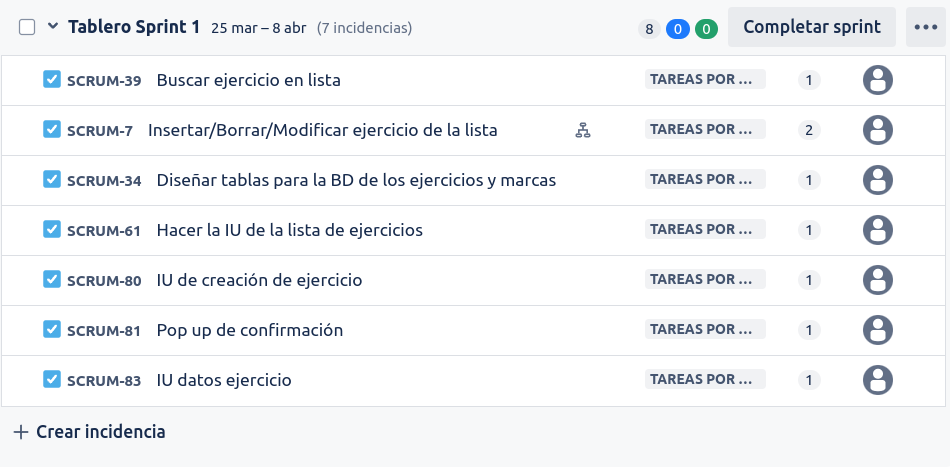
\includegraphics[width=0.7\textwidth]{fotos/PreSrprint1.png}
  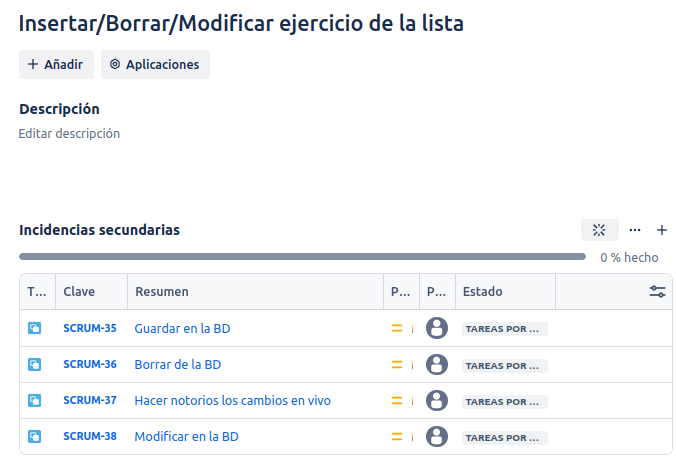
\includegraphics[width=0.7\textwidth]{fotos/SubListPre1.png}
  \caption{Planificacion Sprint 1}
  \label{fig:imagen}
\end{figure}

\subsection{Sprint Review 1}
Estas primeras iteraciones son más lentas porque es el comienzo del desarrollo. No he podido completar la totalidad del sprint, me faltó la subtaread de modifciar ejercicio en la BD. Aun así son buenas las espectativas del desarrollo, dado que la velocidad de desarrollo va a aumentar.

\begin{figure}[h!]
  \centering
  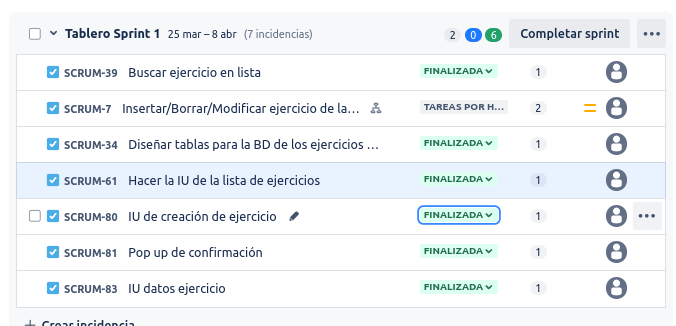
\includegraphics[width=0.7\textwidth]{fotos/PostSprint1.png}
  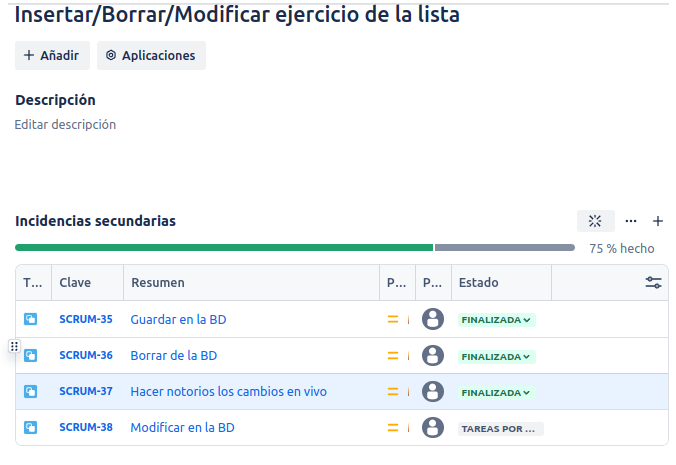
\includegraphics[width=0.7\textwidth]{fotos/SubListPost1.png}
  \caption{Fin Sprint 1}
  \label{fig:imagen}
\end{figure}

En este Sprint review hemos decidido corregir el diseño de la pantalla a uno más intuitivo y cómodo para la vista:

\begin{figure}[h!]
  \centering
  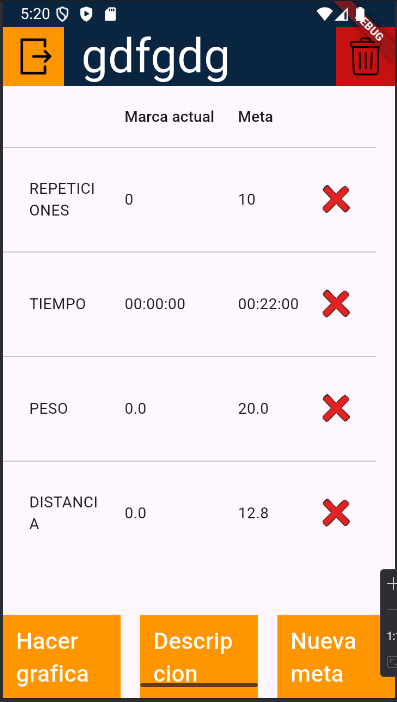
\includegraphics[width=0.4\textwidth]{fotos/ejerciciosNueva.png}
  \caption{Pantalla nueva}
  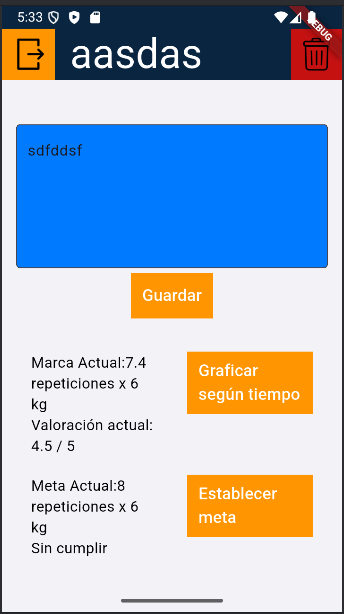
\includegraphics[width=0.4\textwidth]{fotos/ejerciciosVieja.png}
  \caption{Pantalla vieja}
  \label{fig:imagen}
\end{figure}

